\documentclass{article}
\usepackage[utf8]{inputenc}
\usepackage[T1]{fontenc}
\usepackage{booktabs}
\usepackage{graphicx}
\usepackage{hyperref}
\usepackage{xcolor}
\definecolor{validated}{HTML}{047857}
\definecolor{refuted}{HTML}{B91C1C}
\definecolor{inconclusive}{HTML}{9A3412}
\title{Empirical Proof Record: VALIDATED}
\date{2026-05-17T16:40:40.864594+00:00}
\begin{document}
\maketitle
\section*{Empirical Proof Record --- \textcolor{validated}{\textbf{VALIDATED}}}
\textbf{Proof ID:} \texttt{1bc36bbeb4b5c33785a90a4d6c669cf8\dots}\\
\textbf{Created:} 2026-05-17T16:40:40.864594+00:00
\subsection*{1. Claim}
\begin{quote}For Walker M4 events (substrate decision-points: `halt\_reason == 'lateral\_leap'` OR `walker\_annealing\_events > 0`) in a Family J Takwin trajectory, the three-term conservation ratio R = median|Δ(P+T+CW\_seed)| / median|P+T+CW\_seed| is < 0.10. The Phase 137 SEED of scar\_coherence\_weight (`0.5 + 0.5 · \_prior\_trajectory\_coherence`, before Phases 148-182 modulations) is the substrate's clean linear compensator at decision-points. Pressure and tension are averages over named proxy fields per the Sinew Phase 0 inventory (5 pressure + 5 tension); CW\_seed is the legacy `scar\_coherence\_weight` field on OrchestratorResult. All inputs std-normalized before summing.\end{quote}
\begin{itemize}
\item \textbf{Operationalisation:} Auto-detect Walker M4 events per cycle from the trajectory's events dict (lateral\_leap halt OR walker\_annealing\_events > 0). For each event at index i > 0, compute residual = total(i-1) − total(i) where total = norm(P\_avg) + norm(T\_avg) + norm(CW\_seed). Headline metric = median|residual| / median|total|. Bootstrap 95\% CI from 2000 resamples. Verdict on R < threshold. Secondary characterizations: ouroboros + scar conservation ratios + scar magnitude quartile leak structure.
\item \textbf{Threshold:} \texttt{walker\_m4\_conservation\_ratio < 0.1 dimensionless}
\item \textbf{H0:} walker\_m4\_conservation\_ratio >= 0.10 — the substrate does not obey (P+T+CW\_seed) conservation at decision-points; Sinew Phase 4-extended STRONG\_PASS regressed; substrate decision-points fail to compensate stress redistribution within the three-term accounting
\item \textbf{H1:} walker\_m4\_conservation\_ratio < 0.10 — substrate decision-points conserve stress at the STRONG threshold; the Phase 137 SEED is doing genuine compensatory work; Sinew Phase 4-extended finding validated at this commit
\end{itemize}
\subsection*{2. Verdict}
\textcolor{validated}{\textbf{VALIDATED}} --- observed \texttt{0.08734077535187149}\\
Conservation analysis (500 cycles, 105 walker\_m4 events / 35 ouroboros / 465 scar): walker\_m4 R=0.0873 [CI 0.0739, 0.1123]; ouroboros R=0.1163; scar R=0.1048. Scar Q4-leak structure: Q1\_smallest=0.0590, Q2=0.0797, Q3=0.1147, Q4\_largest=0.2067.
\begin{figure}[h!]\centering
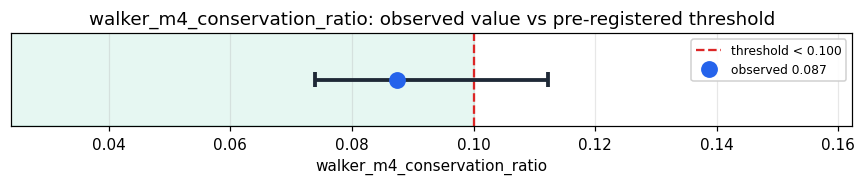
\includegraphics[width=0.8\linewidth]{assets/ci_walker_m4_conservation_ratio}
\caption{walker\_m4\_conservation\_ratio -- observed value with Wilson 95\% CI.}
\end{figure}
\subsection*{3. Evidence}
\begin{tabular}{llrrl}\toprule
\textbf{Pillar} & \textbf{Statistic} & \textbf{Value} & \textbf{95\% CI} & \textbf{Library} \\\midrule
\texttt{sinew\_conservation} & \texttt{walker\_m4\_conservation\_ratio} & \texttt{0.08734077535187149} & (0.0739, 0.1123) & ophamin.measuring.scenarios.sinew\_conservation 0.8.5 \\
\bottomrule\end{tabular}
\subsection*{4. Pre-registration}
\begin{itemize}
\item Registered at: \texttt{2026-05-17T16:40:40.658479+00:00}
\item Config hash: \texttt{9dd6ebb8fde1dec769b834e74bfc353f\dots}
\item Data hash: \texttt{6f7dbd3b70e63ebf77f930d98f0d566d\dots}
\end{itemize}
\subsection*{5. Signature}
\texttt{16ed28c491801a914cc628c62638ea2348b8de4dc96057ff58a3ad50c8d009f0}\\

\end{document}
